% !TEX root = ./rep.tex
\section{Demonstration simulation}
\label{s:demo}

To demonstrate the new capability of Cardinal we demonstrate here the use of
Cardinal on Summit to perform coupled multi-physics simulations of pebble beds.

\subsection{Numerical Setup}

The case presented here comprises 1568 pebbles. The pebble configuration has been obtained using a discrete element method (DEM) code~\cite{projectChronoWebSite}. 
A major overhaul on the mesh generation for the fluid domain has been necessary to automate the process as much as possible and reduce the number of elements per pebble.
te that NekRS shares a similar verification and validation basis with Nek5000
The new meshing tool is based on a Voronoi cell strategy. 
It has allowed for the production of high quality hexahedral meshes, while reducing the element count to roughly 300-400 elements per pebble.

Examples for these meshes are provided in \autoref{f:ndemo1} for the 1568 pebble configuration and in \autoref{f:ndemo2} for a pebble configuration with over 3,000 pebbles.
Both meshes have a similar density.
We note that 1568 pebbles is a significant size for a coupled calculation and representative for instance of the SANA experiments.

\begin{figure}[htb!]
\centering
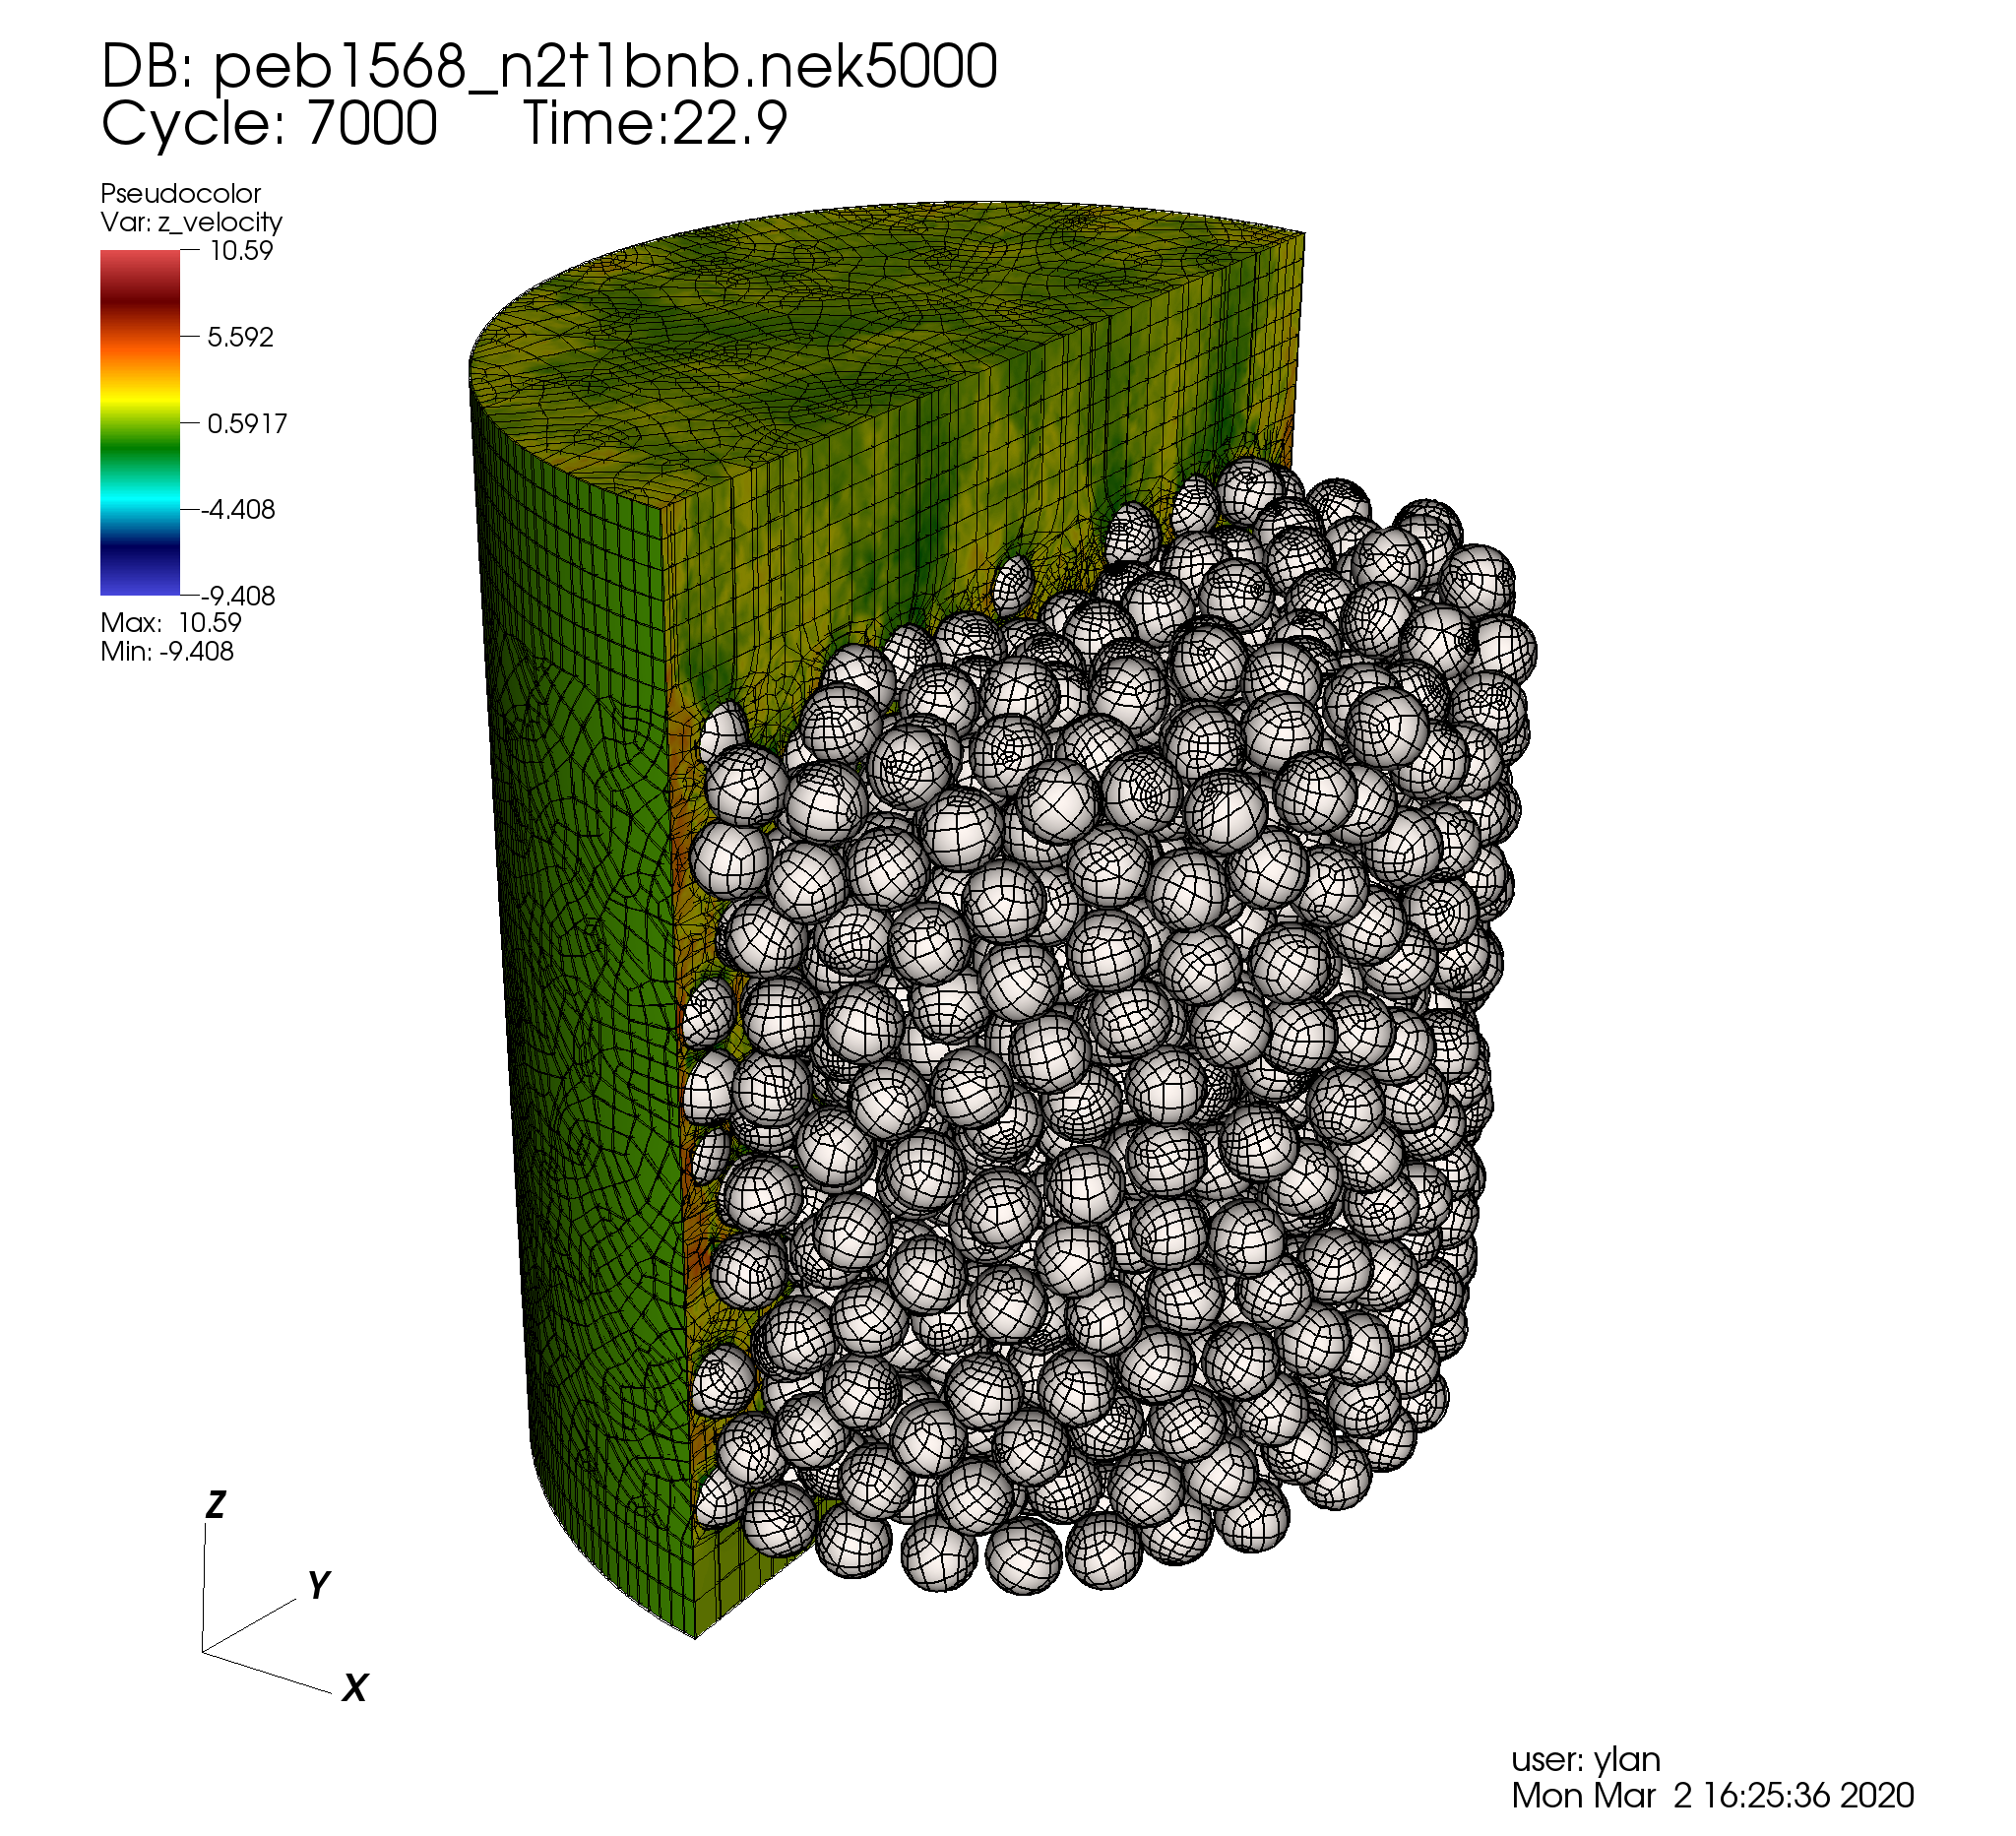
\includegraphics[clip=true,width=0.9\textwidth]{Figures/ndemo_r1}
\caption{NekRS mesh for 1568 pebble configuration using 524,386 spectral elements.}
\label{f:ndemo1}
\end{figure}

\begin{figure}[htb!]
\centering
\includegraphics[clip=true,width=0.9\textwidth]{Figures/ndemo_r2}
\caption{NekRS mesh for 3260 pebble configuration using 1,121,214 spectral elements.}
\label{f:ndemo2}
\end{figure}

The principal objective of the new meshing strategy is to reduce the overall element count so that higher polynomial orders (e.g., $N=7$ to $9$) may be effectively employed.
The base elements for the spectral element method are curvilinear hexahedral (hex) elements with an effective resolution of $N^3$ points for each of $E$ elements.
A minimum value of $n \approx EN^3$ is required to capture the turbulent thermal transport.
With a lower element count, $E$, it is possible to elevate the local approximation order.
$N=7$ is a nearly optimal value for Nek5000/NekRS because it realizes high throughput with reasonable element counts and reasonable time step sizes~\cite{fischer20a}.

The foundation for the new all-hex meshing strategy is to construct the Voronoi tessellation of the thermal-fluid domain in the void space between the spheres and vessel walls.
The Voronoi tessellation has several important properties:
\begin{itemize}
  \item Each Voronoi cell is convex and closed, with cell walls formed by facets that bisect the line connecting adjacent sphere centers.
  \item Each facet is a planar convex polygon.
  \item For $\cal N$ spheres, Voronoi tessellation has an expected complexity of $O(\cal N)$.  
\end{itemize}
Each convex polygon can be tessellated into a set of quadrilaterals if we permit insertion of a vertex along edges.
For example, if the facet is a triangle, we insert a vertex on each of the three edges and then subdivide the triangle into three quads.
Each of these quads can be projected onto the sphere surface to produce a hex element that connects the surface to the Voronoi-cell facet.
For a given sphere, one can refine in the radial direction without having the refinement propagate through the domain.
The same procedure can be performed for each Voronoi cell (i.e., sphere), so the overall complexity is $O(\cal N)$.

Despite the provably good properties of this approach, a significant concern is that the Voronoi tessellation my still contain very thin facets (i.e., {\em slivers}) that lead to poorly conditioned elements.
To overcome this and to generate a more uniform mesh that has a bounded ratio of longest to shortest edge we first perform edge collapse on the Voronoi cells.
Any edge that is shorter than a given tolerance is collapsed and its two vertices are fused into one.
If, after edge collapse, the number of edges on a facet is $<$ 3, the facet is deleted.
Subsequent to edge collapse, we use {\em vertex insertion} to ensure that the {\em longest} edge is below a certain threshold.
The risk of edge collapse is that facets lose their planarity and, worse, might not actually face the sphere that they are nominally bounding.
These situations require some care to recover to ensure that the resulting all-hex mesh has valid positive Jacobians for each element.

Once the mesh is constructed, it is smoothed using a combination of Laplacian smoothing and element-Jacobian optimization where the objective function
includes a substantial penalty for negative Jacobians.

For these demonstrations, the sizes and composition of the TRISO particles were based on TRISO manufactured at INL, following the practice established in the previous report \cite{cardinal}.
Though these particles were developed for the Advanced Gas Reactor (AGR) fuel, particles with the same specifications are used for FHR test reactors and computation benchmarks.
The sizes and compositions of the pebbles were taken from the Mk1 PB-FHR reactor constructed at UC Berkeley.

For BISON, and the demonstration problem under consideration, we consider only the conduction equation and as such it is a relatively straightforward setup.
Properties are constant and adapted from available correlations.
The mesh for a single sphere is generated and replicated at run time.
The same mesh is used for the mesh tallies in OpenMC.

\subsection{Results}

The model described in the previous section has been run on 12 and 20 nodes of Summit, with 6 MPI ranks on each node, corresponding to the 6 GPUs on each node.
The OpenMC and BISON models are designed to run on the CPU while the NekRS model runs on the GPU.

Stand-alone NekRS simulations have been run first up to 25 convective time units to develop turbulence - \autoref{f:ndemo3} using an LES approach.
A restart file has then been generated and used to restart a transient simulation in Cardinal representing a heat-up of the pebbles.
The time step has been fixed to $5(10^{-4})$s in both BISON and NekRS.
The temperature at time zero has been set to $300\degree$C everywhere.
\autoref{f:ndemo4} presents the temperature at the surface of the pebbles in BISON at three points in time.
The simulations took 2.5s per coupled time step on 20 nodes, requiring transfer between physics at each time step.
However, this could be greatly optimized by relaxing the requirement, as data transfer from GPU to CPU should be minimized as much as possible.

\begin{figure}[htb!]
\centering
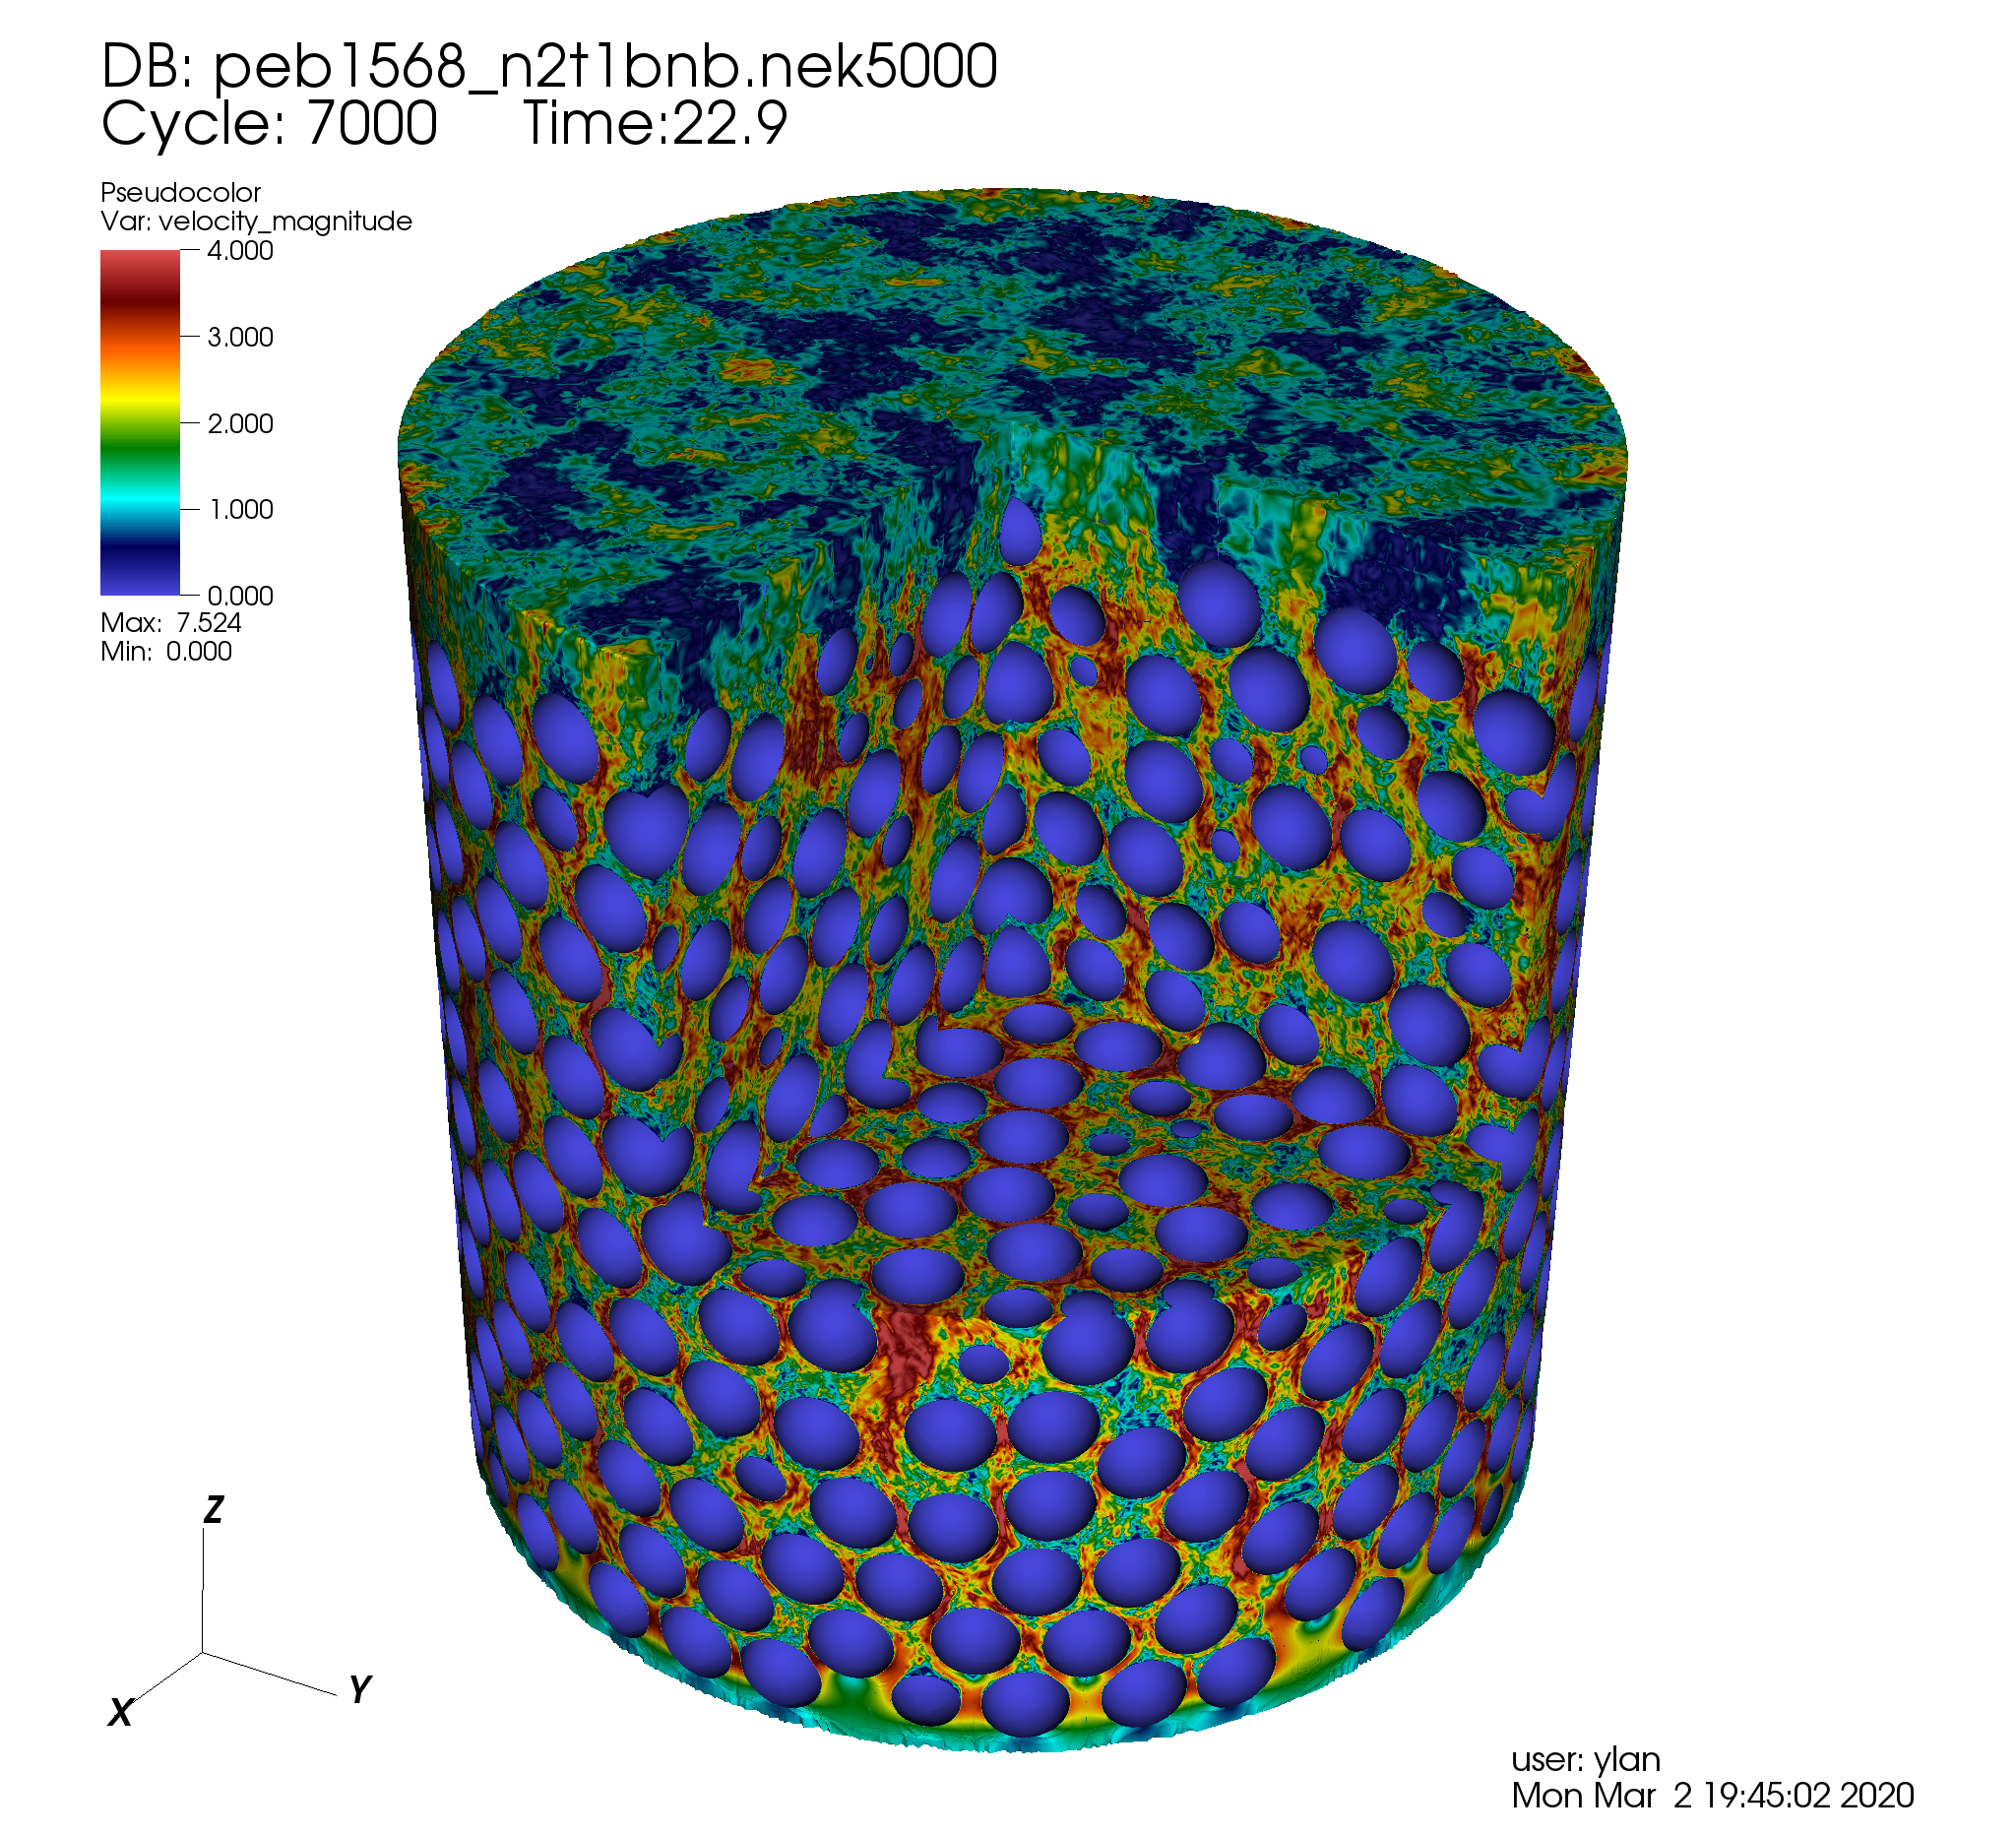
\includegraphics[clip=true,width=0.9\textwidth]{Figures/ndemo_r3}
\caption{NekRS results for the velocity field.}
\label{f:ndemo3}
\end{figure}


\begin{figure}[htb!]
\centering
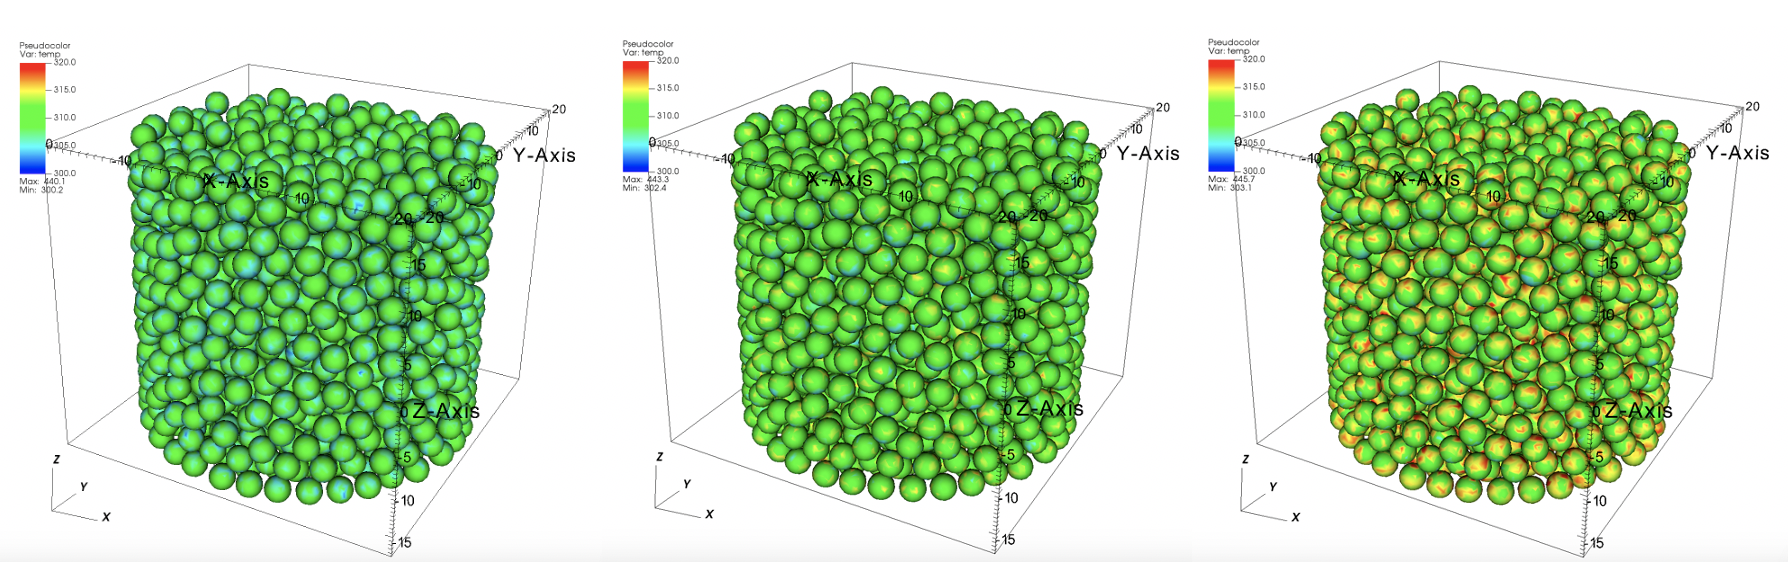
\includegraphics[clip=true,width=0.9\textwidth]{Figures/ndemo_r4}
\caption{Temperature result for the pebble surface temperature at three points in time.}
\label{f:ndemo4}
\end{figure}

The results of OpenMC simulations coupled with the heat conduction module are shown in \autoref{f:1568_openmc_heat_source} and \autoref{f:1568_openmc_temperatures} with the same time step parameters as the NekRS simulations described above.
An eigenvalue simulation using 150 batches with 50 inactive batches was executed in each time step.
50,000 particles per batch were used to converge the pebble-averaged heat source from the OpenMC cell tally while the unstructured mesh heat source tally required 500,000 particles per batch to produce the heat source presented here.
Production simulations may require an even higher number of particles per batch to more tightly converge the heating distribution when using the unstructured mesh heat source due to the decreased number of samples per source particle in the tally bins.
\autoref{f:1568_openmc_temperatures_single_pebble} demonstrates the effect of the improved spatial resolution provided by the unstructured mesh heat source from OpenMC on the temperature distribution within a representative pebble.
In the case of the pebble-averaged heat source the temperature profile is symmetric.
This reflects the uniform heat source applied in that region.
An asymmetry can be seen in the profile generated from the unstructured mesh heat source, indicating that the improved spatial resolution of the source has an impact on the temperature distribution in the solid.
This will in turn affect the resulting heat transfer to the fluid.

\begin{figure}[htb!]
\centering
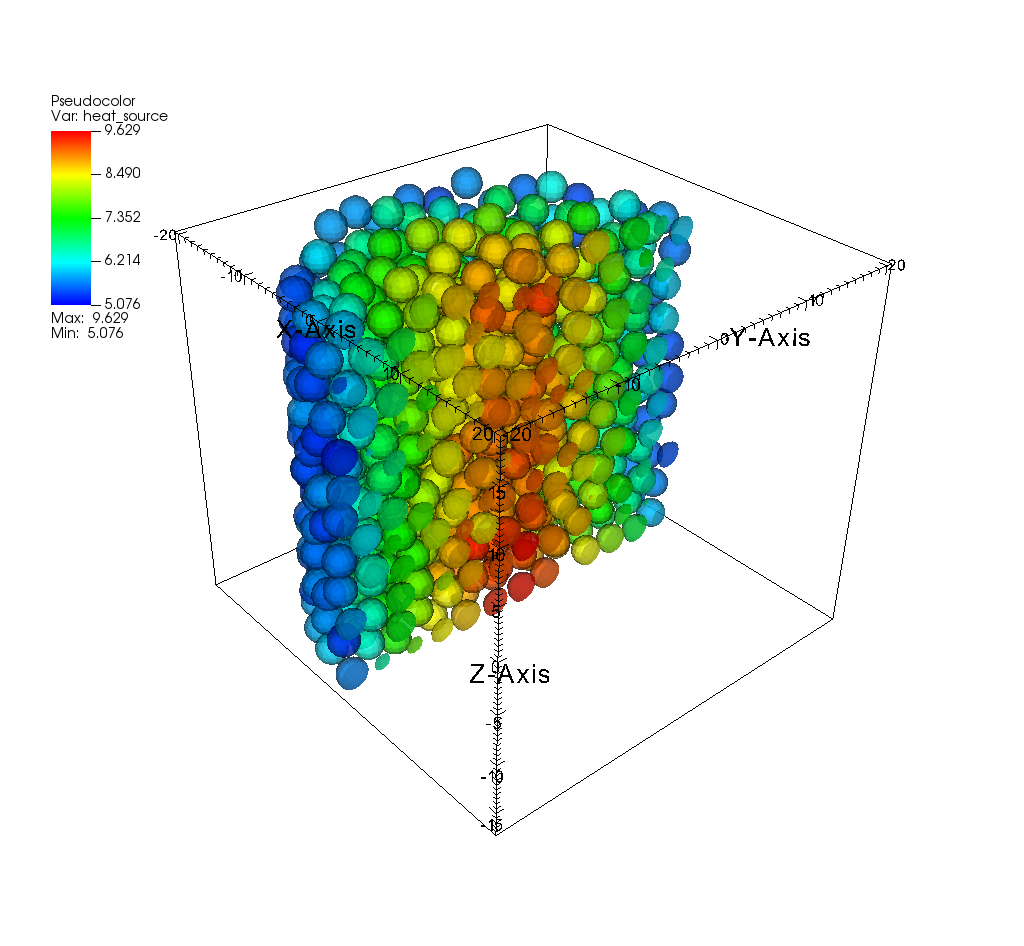
\includegraphics[clip=true,width=0.48\textwidth]{Figures/openmc_cell_heat_source}
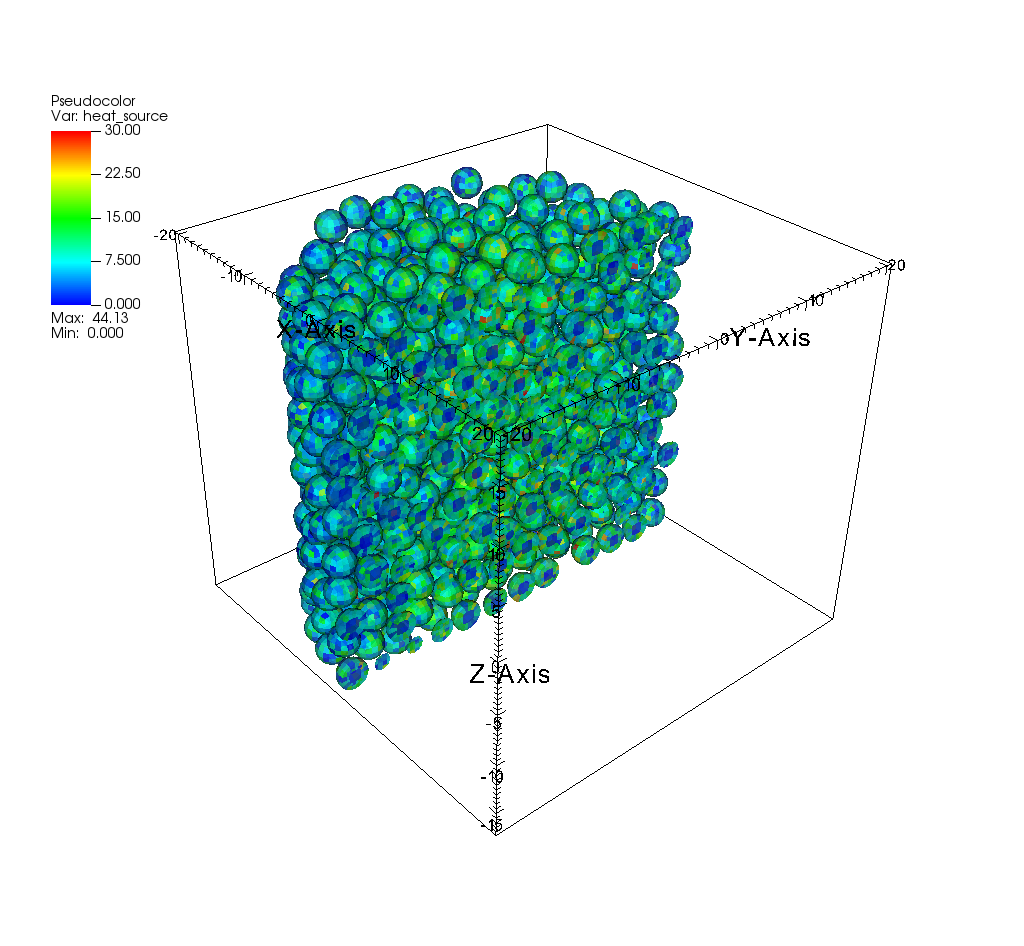
\includegraphics[clip=true,width=0.48\textwidth]{Figures/openmc_mesh_heat_source}
\caption{Left: Heat source using the original cell tallies to produces an average heat source per-pebble. Right: Heat source produced using an OpenMC unstructured mesh tally.}
\label{f:1568_openmc_heat_source}
\end{figure}

\begin{figure}[htb!]
\centering
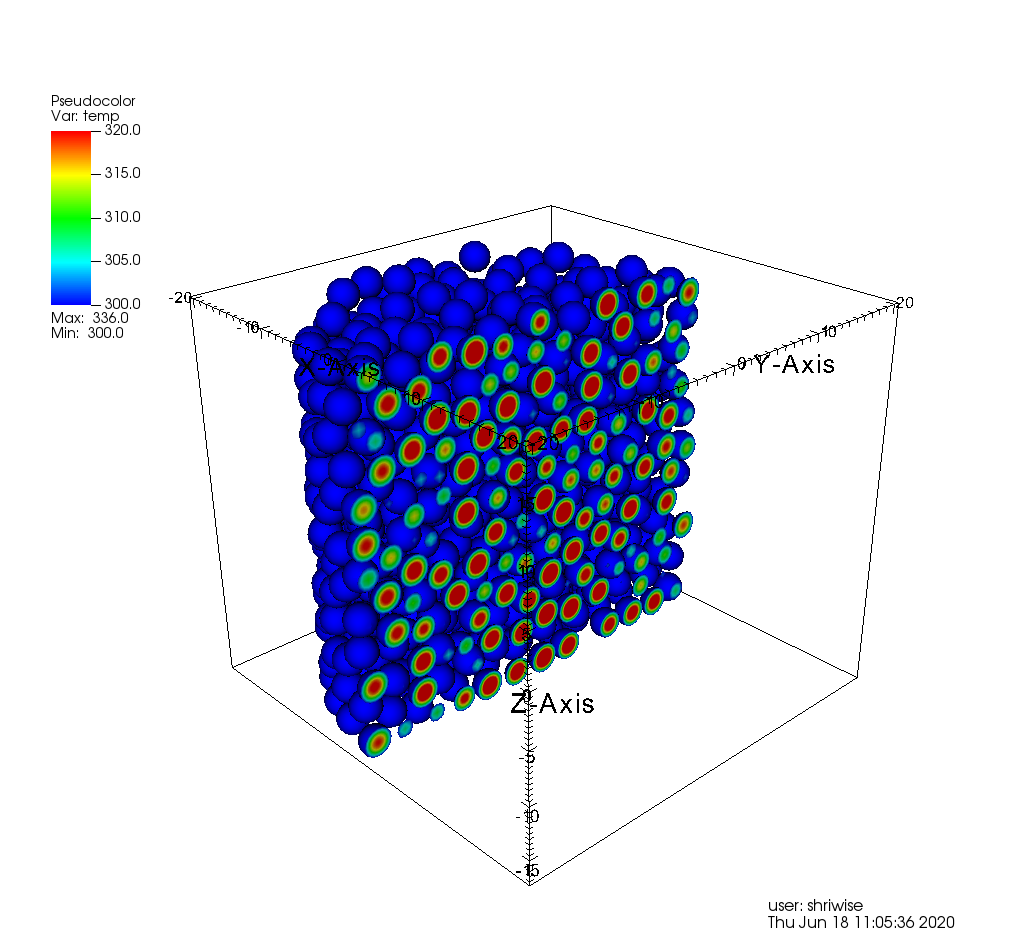
\includegraphics[clip=true,width=0.48\textwidth]{Figures/openmc_cell_temperature}
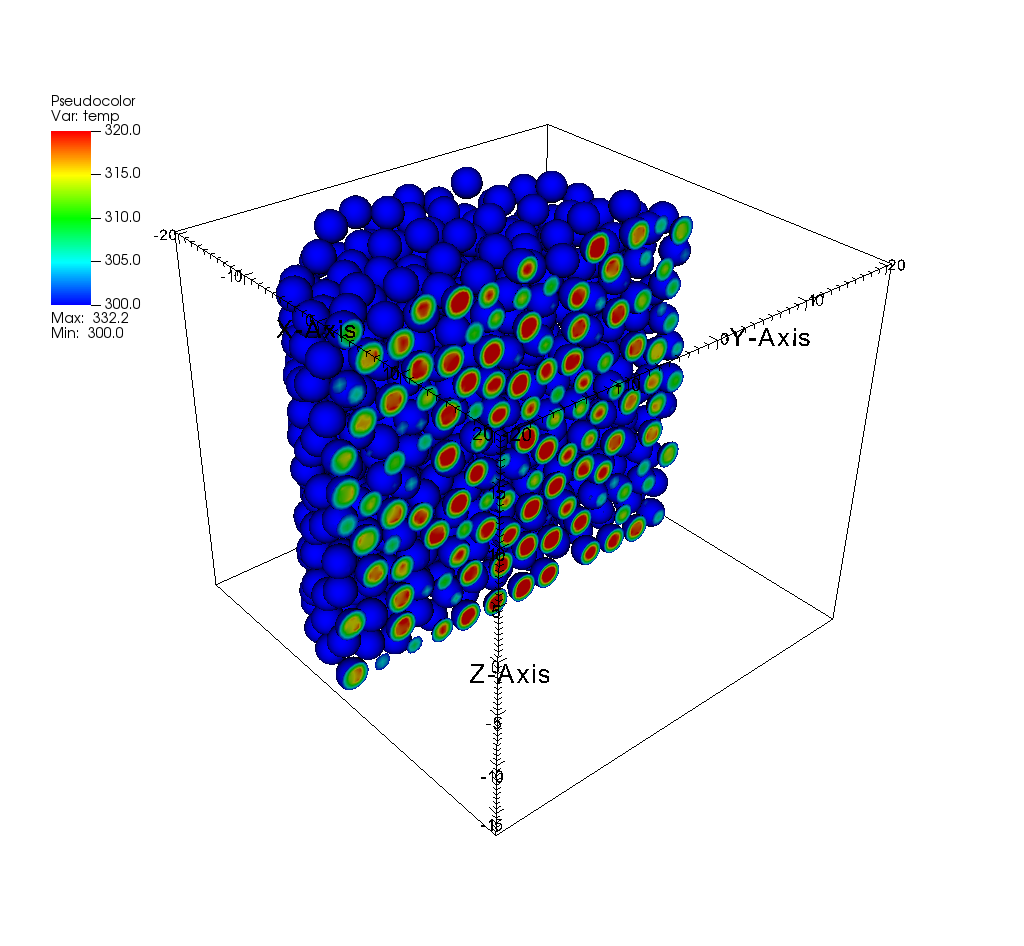
\includegraphics[clip=true,width=0.48\textwidth]{Figures/openmc_mesh_temperature}
\caption{Left: Temperature in the solid resulting from the cell-based heating tally. Right: Temperature in the solid resulting from the unstructured mesh heating tally in OpenMC.}
\label{f:1568_openmc_temperatures}
\end{figure}

\begin{figure}[htb!]
\centering
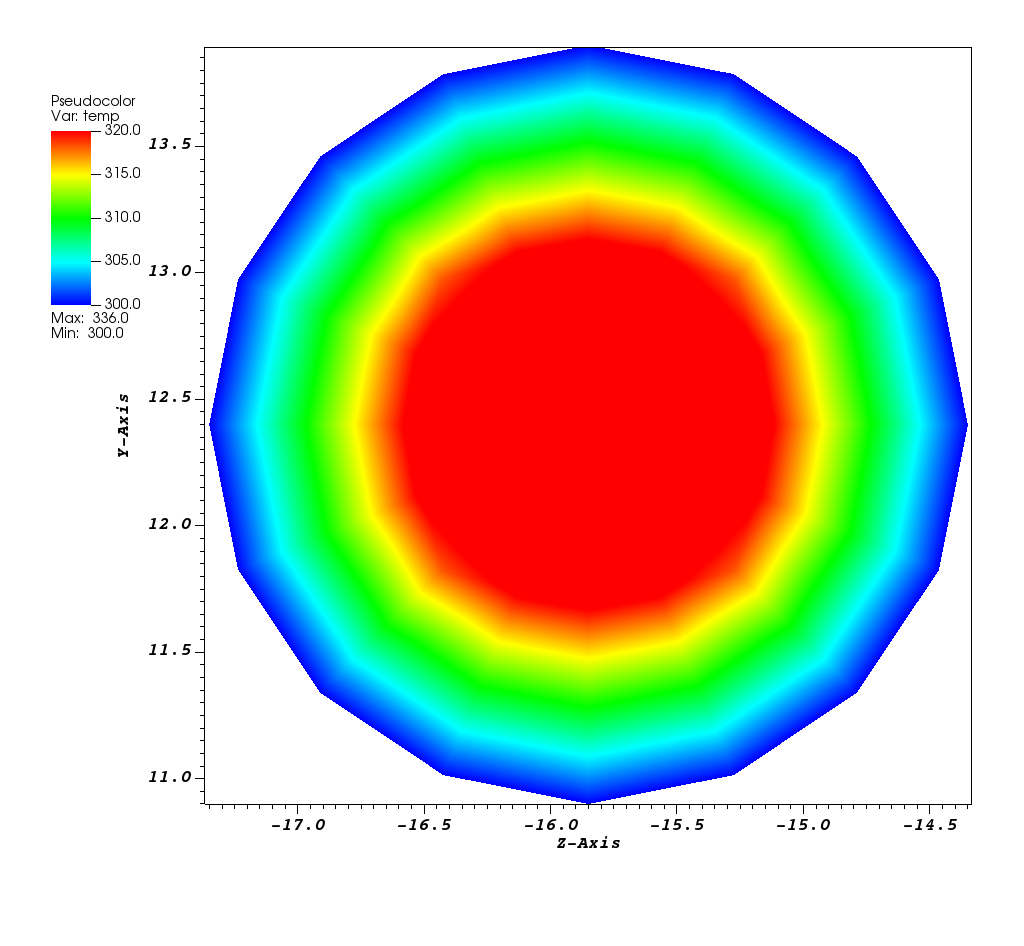
\includegraphics[clip=true,width=0.48\textwidth]{Figures/openmc_cell_temperature_zoomed}
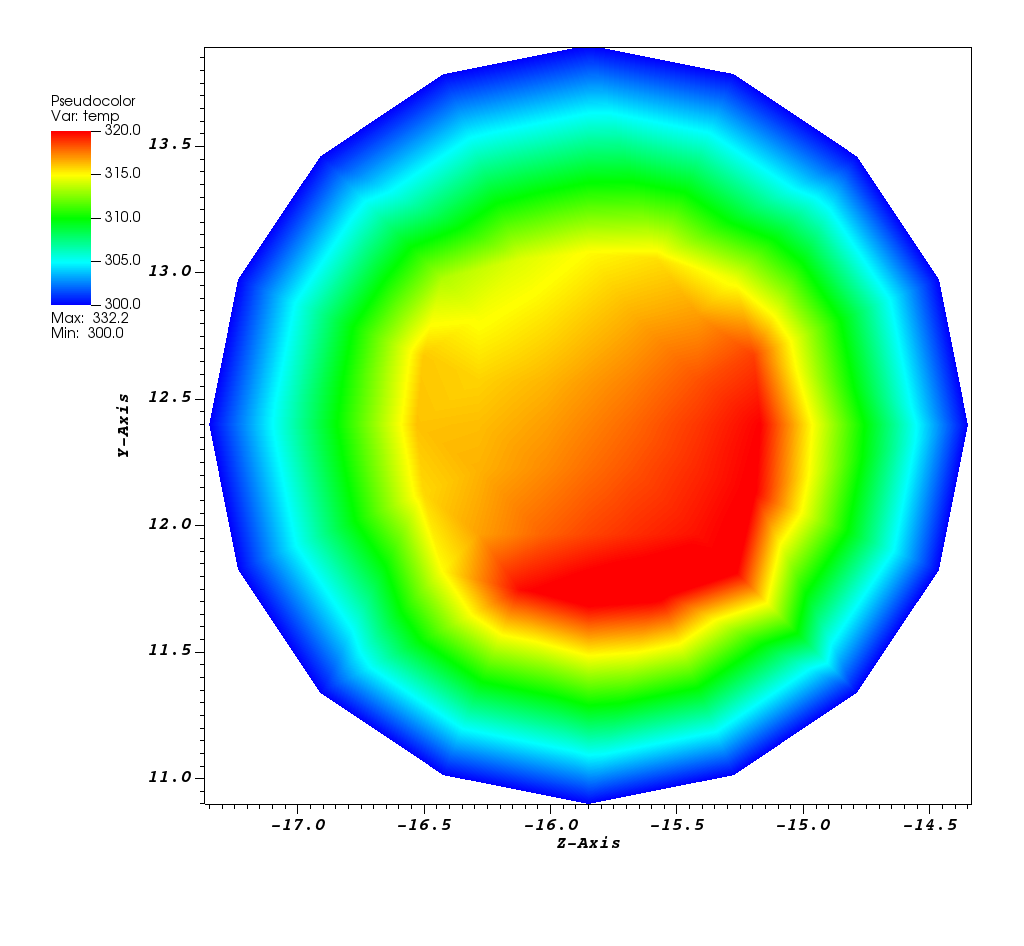
\includegraphics[clip=true,width=0.48\textwidth]{Figures/openmc_mesh_temperature_zoomed}
\caption{Temperature profiles of the same pebble in the 1568 pebble demo using the pebble-averaged heating (left) and the unstructured mesh heating (right).}
\label{f:1568_openmc_temperatures_single_pebble}
\end{figure}

\subsection{Projection to full core}

20 nodes of Summit represents less than 1\% of the computing power available on Summit.
We estimate that 80\% of the machine will be sufficient to perform full core calculations in FHRs corresponding to 300,000 pebbles.
